\documentclass{article}

\usepackage{amsmath,amssymb}
\usepackage{tikz}
\usepackage{pgfplots}
\usepackage{xcolor}
\usepackage[left=2.1cm,right=3.1cm,bottom=3cm,footskip=0.75cm,headsep=0.5cm]{geometry}
\usepackage{enumerate}
\usepackage{enumitem}
\usepackage{marvosym}
\usepackage{tabularx}
\usepackage{tikz-qtree}
\usetikzlibrary{patterns,arrows,calc,decorations.pathmorphing,backgrounds, positioning,fit,petri,decorations.fractals,trees,cd,automata,babel,shapes.geometric,arrows.meta,bending}

\usepackage[utf8]{inputenc}

\renewcommand*{\arraystretch}{1.4}

\newcolumntype{L}[1]{>{\raggedright\arraybackslash}p{#1}}
\newcolumntype{R}[1]{>{\raggedleft\arraybackslash}p{#1}}
\newcolumntype{C}[1]{>{\centering\let\newline\\\arraybackslash\hspace{0pt}}m{#1}}

\title{\textbf{Steuertheorie, Hausaufgabe 6}}
\author{\textsc{Henry Haustein}}
\date{}

\begin{document}
	\maketitle
	
	\section*{Aufgabe 1}
	\begin{enumerate}[label=(\alph*)]
		\item Johansson-Samuelson-Theorem: Ein Steuersystem mit Ertragswertabschreibung lässt die Ertragswerte unverändert und verzerrt damit die Investitionsentscheidung nicht.
		\item Es gilt
		\begin{align}
			E_0 &= \frac{300}{1+0.05} + \frac{2000}{(1+0.05)^2} = 2099.77 \notag \\
			E_1 &= \frac{2000}{1+0.5} = 1904.76 \notag \\
			E_2 &= 0 \notag
		\end{align}
		\item Für die Steuerabschreibung gilt: $a_t=-\Delta E_t$, also
		\begin{align}
			a_1 &= -(E_1-E_0) = -(1904.76-2099.77) = 195.01 \notag \\
			a_2 &= -(E_2-E_1) = -(0-1904.76) = 1904.76 \notag
		\end{align}
	\end{enumerate}

	\section*{Aufgabe 2}
	\begin{enumerate}[label=(\alph*)]
		\item Die Grenzprodukte sind
		\begin{align}
			GP_A &= 10-K_A \notag \\
			GP_B &= 10-\frac{1}{2}K_B \notag
		\end{align}
		\begin{center}
			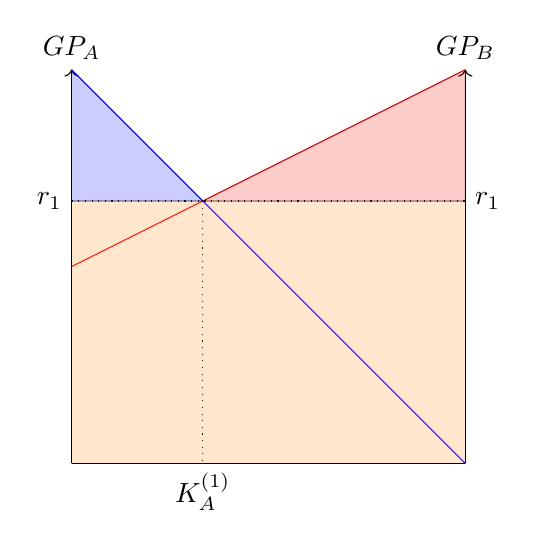
\begin{tikzpicture}
				\draw[->] (0,0) -- (0,5) node[above] {$GP_A$};
				\draw (0,0) -- (5,0);
				\draw[->] (5,0) -- (5,5) node[above] {$GP_B$};
				
				\draw[blue] (0,5) -- (5,0);
				\draw[red] (5,5) -- (0,2.5);
				
				\draw[dotted] (0,10/3) node[left] {$r_1$} -- (5,10/3) node[right] {$r_1$};
				\draw[dotted] (5/3,10/3) -- (5/3,0) node[below] {$K_A^{(1)}$};
				
				\draw[fill=orange,opacity=0.2] (0,0) rectangle (5,10/3);
				\draw[fill=blue,opacity=0.2] (0,5) -- (0,10/3) -- (5/3,10/3) -- (0,5);
				\draw[fill=red,opacity=0.2] (5,5) -- (5,10/3) -- (5/3,10/3) -- (5,5);
			\end{tikzpicture} \\
			\textcolor{blue}{$GP_A$ mit Bodenrente in A}, \textcolor{red}{$GP_B$ mit Bodenrente in B}, \textcolor{orange}{Kapitaleinkommen}
		\end{center}
		\item Es gilt $GP_A=GP_B$ mit $K_A+K_B=10$, also
		\begin{align}
			GP_A &= GP_B \notag \\
			10-K_A &= 10-\frac{1}{2}(10-K_A) \notag \\
			10-K_A &= 5-\frac{K_A}{2} \notag \\
			5 &= \frac{3}{2}K_A \notag \\
			K_A^{(1)} &= \frac{10}{3} \Rightarrow K_B^{(1)}=\frac{20}{3} \notag
		\end{align}
		Der Zins ist $r=GP_A(K_A)=\frac{20}{3}$.
		\item Die Steuerlast wird hauptsächlich von Bodenbesitzern in A getragen, da das Kapital abfliegt und Kapitalbesitzern, da der Zins sinkt.
		\begin{center}
			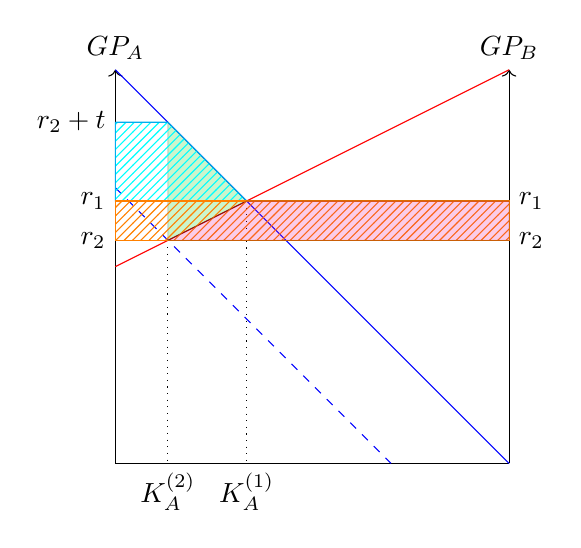
\begin{tikzpicture}
				\draw[->] (0,0) -- (0,5) node[above] {$GP_A$};
				\draw (0,0) -- (5,0);
				\draw[->] (5,0) -- (5,5) node[above] {$GP_B$};
				
				\draw[blue] (0,5) -- (5,0);
				\draw[blue,dashed] (0,3.5) -- (3.5,0);
				\draw[red] (5,5) -- (0,2.5);
				
				\draw[dotted] (0,10/3) node[left] {$r_1$} -- (5,10/3) node[right] {$r_1$};
				\draw[dotted] (0,17/6) node[left] {$r_2$} -- (5,17/6) node[right] {$r_2$};
				\draw[dotted] (2/3,13/3) -- (0,13/3) node[left] {$r_2+t$};
				\draw[dotted] (5/3,10/3) -- (5/3,0) node[below] {$K_A^{(1)}$};
				\draw[dotted] (2/3,17/6) -- (2/3,0) node[below] {$K_A^{(2)}$};
				
				\draw[fill=green!80!black,opacity=0.2] (2/3,17/6) -- (2/3,13/3) -- (5/3,10/3) -- (2/3,17/6);
				\draw[cyan,pattern=north east lines, pattern color=cyan] (0,13/3) -- (2/3,13/3) -- (5/3,10/3) -- (0,10/3) -- (0,13/3);
				\draw[orange,pattern=north east lines, pattern color=orange] (0,10/3) rectangle (5,17/6);
				\draw[fill=magenta,opacity=0.2] (2/3,17/6) -- (5,17/6) -- (5,10/3) -- (5/3,10/3) -- (2/3,17/6);
				
			\end{tikzpicture} \\
			\textcolor{blue}{$GP_A$ ohne/mit Steuern}, \textcolor{red}{$GP_B$}, \textcolor{green!80!black}{Wohlfahrtsverlust}, \textcolor{cyan}{Verringerung der Bodenrente in A}, \textcolor{orange}{Verringerung der Kapitaleinkommen}, \textcolor{magenta}{Erhöhung der Bodenrente in B}
		\end{center}
		\item Es gilt
		\begin{align}
			GP_A - t &= GP_B \notag \\
			10-K_A-t &= 10-\frac{1}{2}K_B \notag \\
			10-K_A-t &= 10-\frac{1}{2}(10-K_A) \notag \\
			10-K_A-t &= 5+\frac{K_A}{2} \notag \\
			5-t &= \frac{3}{2}K_A \notag \\
			K_A^{(2)} &= \frac{10}{3}-\frac{2}{3}t \notag
		\end{align}
		Der Kapitalabfluss ist $K_A^{(1)}-K_A^{(2)}=\frac{2}{3}t$ und das Steueraufkommen ist $T=K_A\cdot t=\frac{10}{3}t - \frac{2}{3}t^2$.
		\item Der Wohlfahrtsverlust ist
		\begin{align}
			WFV &= \frac{1}{2}\left(K_A^{(1)} - K_A^{(2)}\right)\cdot t \notag \\
			&= \frac{1}{3}t^2 \notag
		\end{align}
		Weiterhin gilt
		\begin{align}
			\frac{\partial WFV}{\partial t} = \frac{2}{3}t \quad\text{und}\quad \frac{\partial^2 WFV}{\partial t^2} = \frac{2}{3} \notag
		\end{align}
		Der Wohlfahrtsverlust steigt überproportional mit der Steuer.
		\item Es gilt
		\begin{align}
			\frac{\partial T}{\partial t} &= \frac{10}{3} - \frac{4}{3}t = 0 \notag \\
			\frac{10}{3} &= \frac{4}{3}t \notag \\
			t &= \frac{5}{2} \notag
		\end{align}
		Ist $t<\frac{5}{2}$, so steigt das Steueraufkommen mit steigendem Steuersatz. Ab $t>\frac{5}{2}$ sinkt das Steueraufkommen mit steigendem Steuersatz.
	\end{enumerate}
	
	\section*{Aufgabe 3}
	\begin{enumerate}[label=(\alph*)]
		\item Die Grenzproduktivitäten sind
		\begin{align}
			GP_B &= 20-K_B \notag \\
			GP_A &= \begin{cases}
				z &K_A \le 5 \\
				0 & K_A > 5
			\end{cases} \notag
		\end{align}
		\begin{center}
			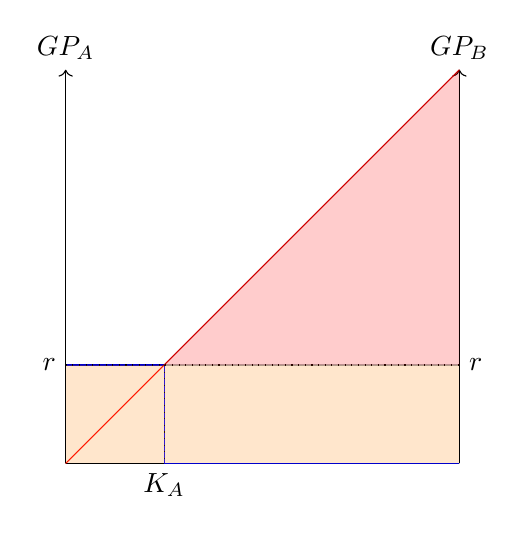
\begin{tikzpicture}
				\draw[->] (0,0) -- (0,5) node[above] {$GP_A$};
				\draw (0,0) -- (5,0);
				\draw[->] (5,0) -- (5,5) node[above] {$GP_B$};
				
				\draw[blue] (0,5/4) -- (5/4,5/4) -- (5/4,0) -- (5,0);
				\draw[red] (5,5) -- (0,0);
				
				\draw[dotted] (0,5/4) node[left] {$r$} -- (5,5/4) node[right] {$r$};
				\draw[dotted] (5/4,5/4) -- (5/4,0) node[below] {$K_A$};
				
				\draw[fill=orange,opacity=0.2] (0,0) rectangle (5,5/4);
				\draw[fill=red,opacity=0.2] (5,5) -- (5,5/4) -- (5/4,5/4) -- (5,5);
			\end{tikzpicture} \\
			\textcolor{blue}{$GP_A$}, \textcolor{red}{$GP_B$ mit Bodenrente in B}, \textcolor{orange}{Kapitaleinkommen}
		\end{center}
		\item Die Nachfrage nach Kapital in A ist vollkommen unelastisch für $0<r\le z$. Für $K_A\le 5$ gilt $GP_G\le GP_F$. Land A wird 5 Einheiten Kapital für $0<r\le z$ nachfragen. Damit die übrigen 15 Kapitaleinheiten nachgefragt werden und somit Markträumung herrscht, muss $r=GP_G(15)$ gelten, also $r=5$.
		\item Die Kapitalaufteilung bleibt unverändert, es gibt keinen Wohlfahrtsverlust
		\begin{center}
			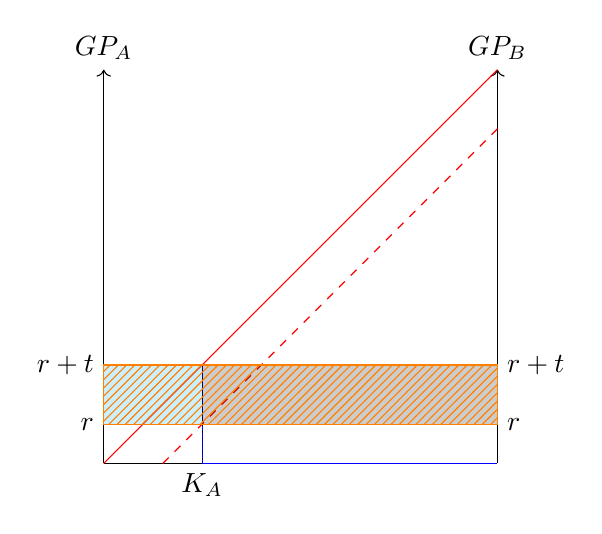
\begin{tikzpicture}
				\draw[->] (0,0) -- (0,5) node[above] {$GP_A$};
				\draw (0,0) -- (5,0);
				\draw[->] (5,0) -- (5,5) node[above] {$GP_B$};
				
				\draw[blue] (0,5/4) -- (5/4,5/4) -- (5/4,0) -- (5,0);
				\draw[red] (5,5) -- (0,0);
				\draw[red,dashed] (5,17/4) -- (3/4,0);
				
				\draw[dotted] (0,5/4) node[left] {$r+t$} -- (5,5/4) node[right] {$r+t$};
				\draw[dotted] (0,0.5) node[left] {$r$} -- (5,0.5) node[right] {$r$};
				\draw[dotted] (5/4,5/4) -- (5/4,0) node[below] {$K_A$};
				
				\draw[fill=black,opacity=0.2] (5/4,5/4) rectangle (5,0.5);
				\draw[fill=cyan,opacity=0.2] (0,0.5) rectangle (5/4,5/4);
				\draw[orange,pattern=north east lines, pattern color=orange] (0,0.5) rectangle (5,5/4);		
			\end{tikzpicture} \\
			\textcolor{blue}{$GP_A$}, \textcolor{red}{$GP_B$ ohne/mit Steuern}, \textcolor{cyan}{Zuwachs Bodenrente in A}, \textcolor{gray}{Steueraufkommen}, \textcolor{orange}{Verringerung Kapitaleinkommen}
		\end{center}
		\item Die Kapitalaufteilung bleibt unverändert, da es sich in A um eine vollkommen unelastische Kapitalnachfrage handelt. Also $K_A=5$, $K_B=15$ und
		\begin{align}
			r + t &= 20-K_B \notag \\
			r+3 &= 5 \notag \\
			r &= 2 \notag
		\end{align}
		\item Das Steueraufkommen ist $T=K_B\cdot t=15\cdot 3=45$ und wird ausschließlich von Kapitalbesitzern in B getragen.
	\end{enumerate}
	
\end{document}